\section{Examples for 2D Reverse Fault with Splay}
\label{sec:example:reverse:2d}

% ----------------------------------------------------------------------
\subsection{Overview}

This suite of examples demonstrates use of a number of features for a
simple two-dimensional model. This example also shows how to produce
a mesh with a somewhat complex geometry. Although the problem geometry
(Figure~\ref{fig:example:reverse:2d:geometry}) includes a simple
planar splay fault intersecting a planar thrust fault, the first 3
steps actually focus on gravitational body forces, reference stresses,
and incompressible elasticity. The fourth example demonstrates the use
of traction boundary conditions to represent a surface load. The
remainder of the examples focus on slip on one or more faults,
including an example of multiple ruptures on a single fault.
To keep the meshing and computation time in these
examples short, we limit our model to a 200 km $\times$ 100 km
domain and we will use a relatively coarse discretization.

\begin{figure}[htbp]
  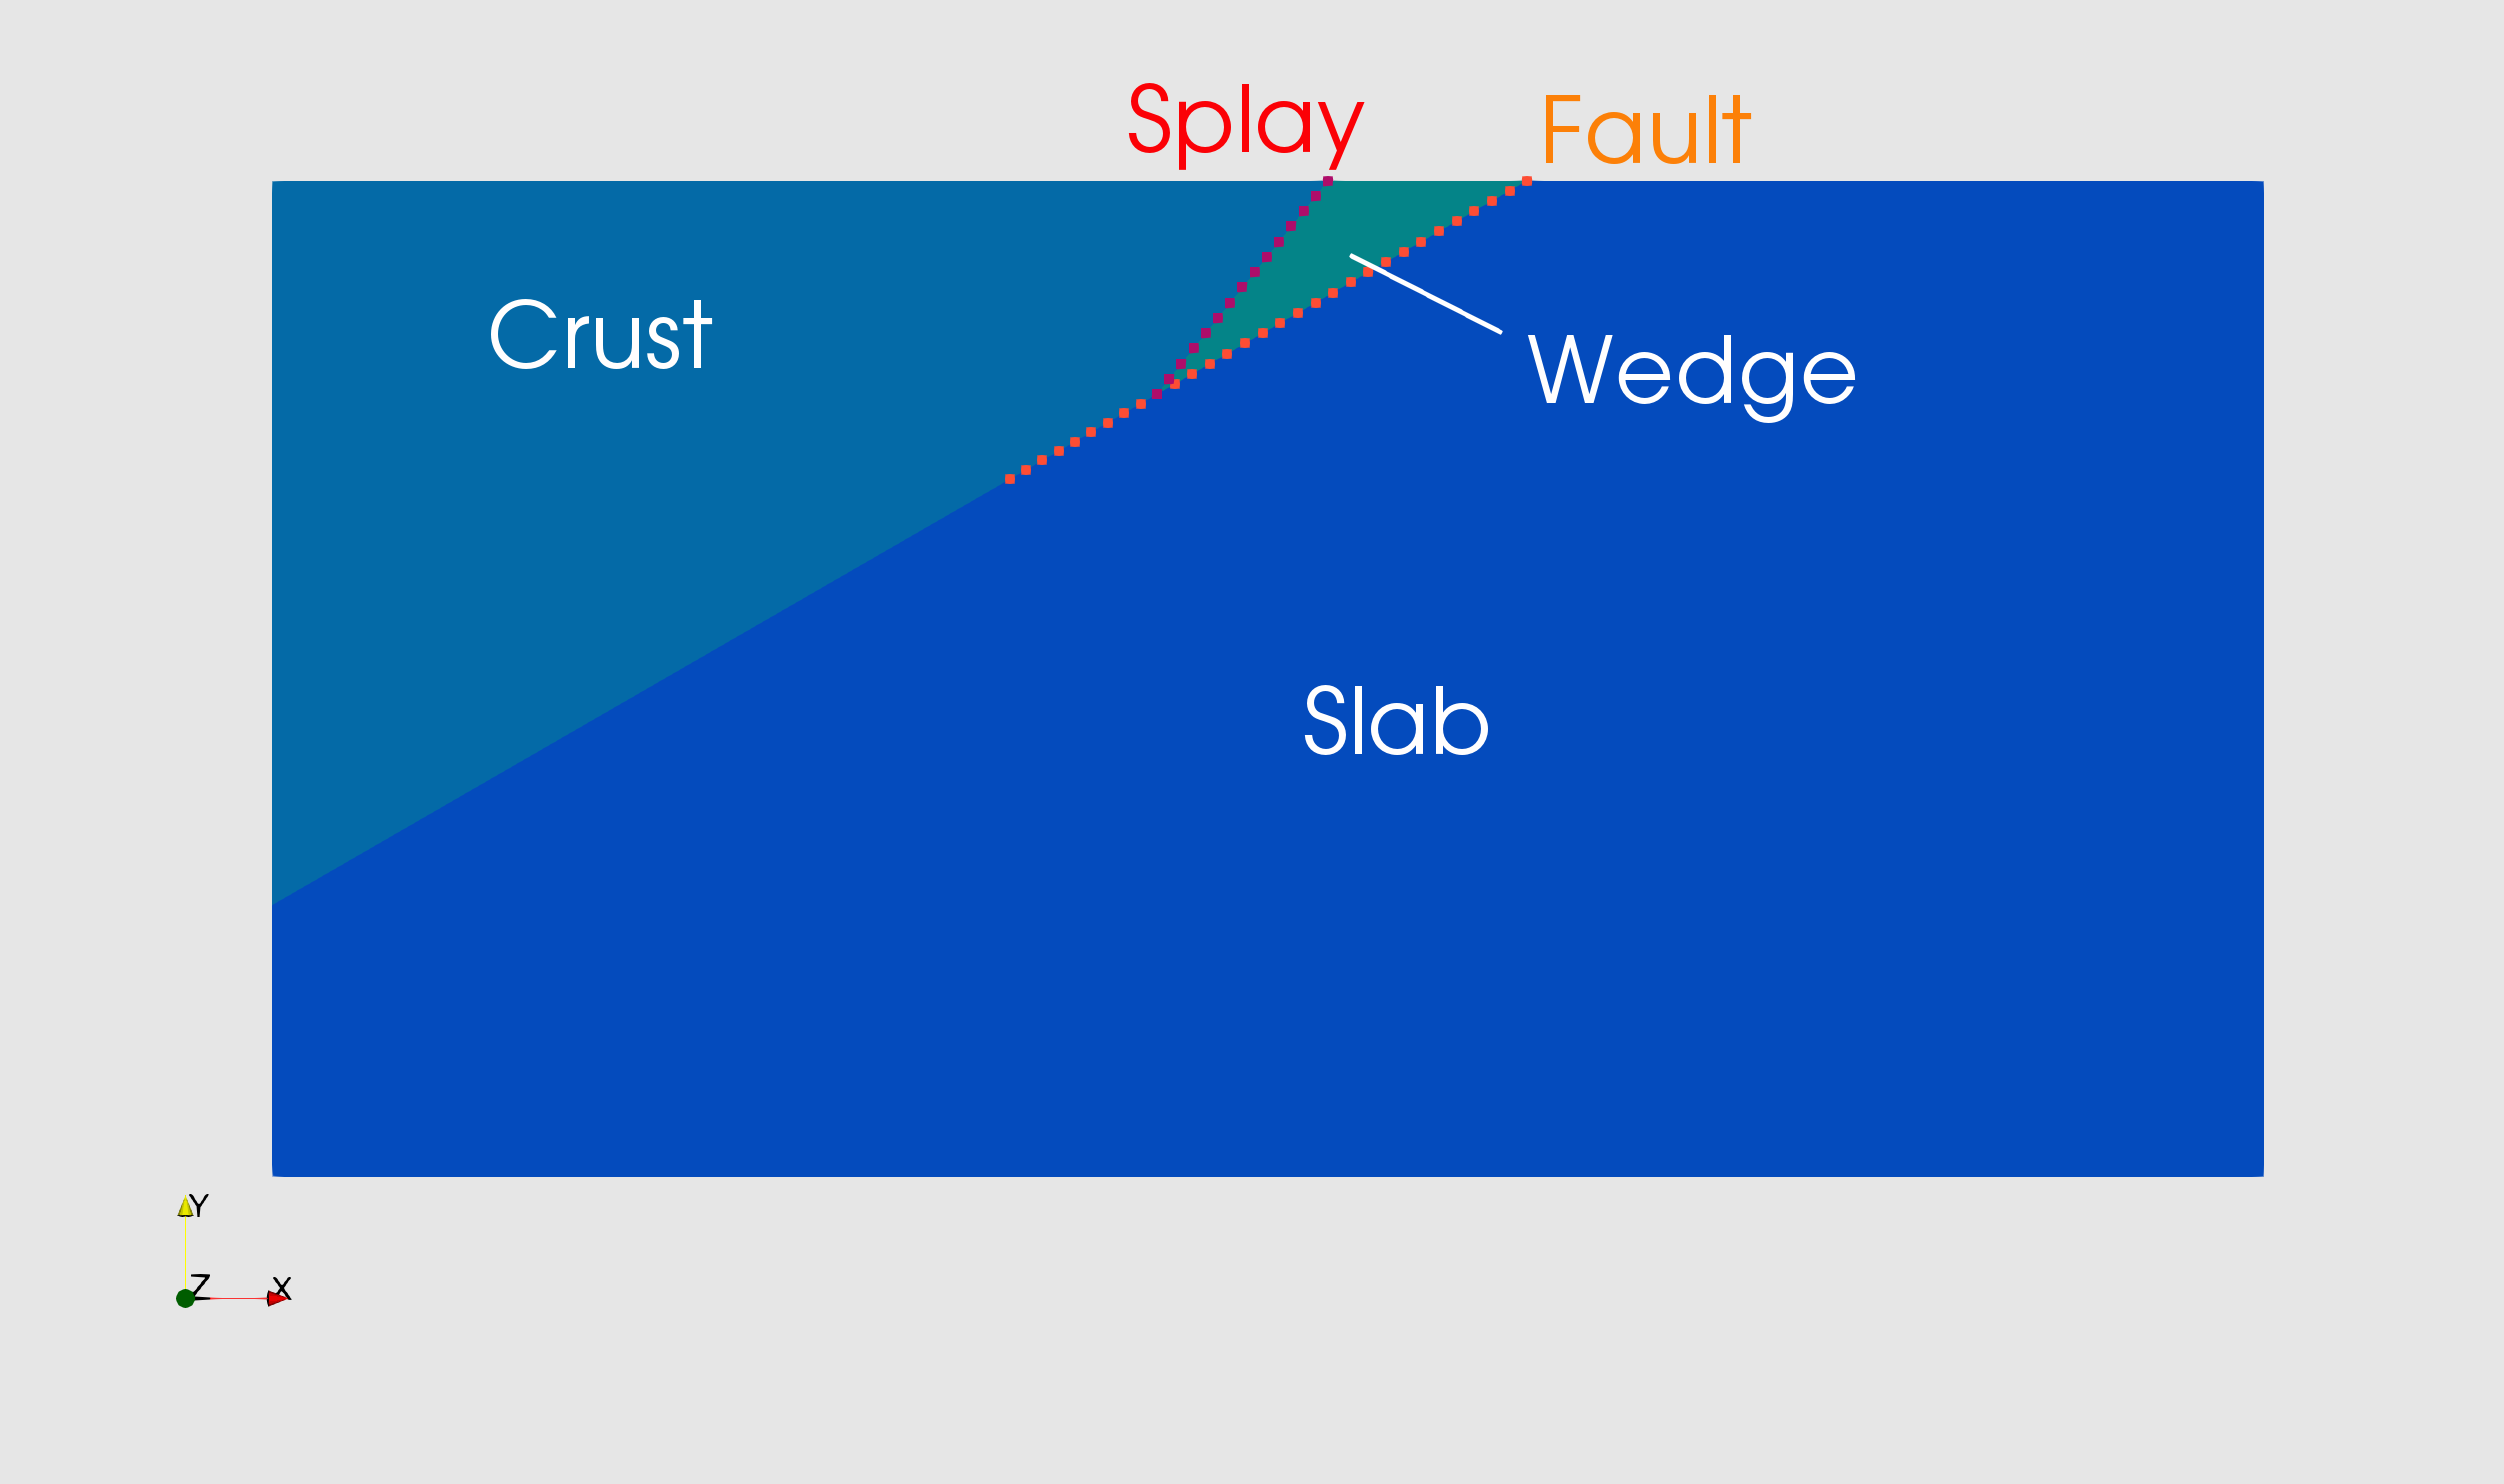
\includegraphics[width=4.5in]{examples/figs/reverse2d_geometry}
  \caption{Geometry used for 2D reverse fault example.}
  \label{fig:example:reverse:2d:geometry}
\end{figure}

Note that although we label the different parts of the mesh as slab,
crust, and wedge, the actual thrust fault only extends 60 km downdip,
and we do not provide bottom boundaries for the crust and slab.
The files associated with this suite of examples are contained in the
directory \filename{examples/2d/reverse}. This directory contains
several files:
\begin{description}
\item[\filename{*.jou}] Files used to construct the finite-element mesh using
  CUBIT/Trelis.
\item[\filename{*.spatialdb}] Files associated with the spatial databases.
\item[\filename{viz}] Directory containing ParaView
  Python scripts and other files for visualizing results.
\item[\filename{output}] Directory containing simulation
  output. It is created automatically when running the
  simulations.
\item[\filename{README.md}] README file containing a brief description
  of the various examples.
\end{description}


% ----------------------------------------------------------------------
\subsection{Features Illustrated}

Table~\ref{tab:example:reverse:2d:features} lists the features
discussed in each of these 2-D reverse fault examples. With the
intent of illustrating features used in research simulations, we use
HDF5 output and we make extensive use the most efficient
implementations of spatial databases (UniformDB and ZeroDB). We
also use ParaView Python scripts for visualizing the output. These
scripts can be run within the ParaView GUI or outside the ParaView
GUI, although the interaction is limited to rotating, translating, and
zooming when run outside the ParaView GUI.

\begin{table}[htbp]
  \caption{PyLith features covered in the suite of 2-D reverse fault examples.}
  \label{tab:example:reverse:2d:features}
  \input{examples/2d_reverse_features}
\end{table}

% ----------------------------------------------------------------------
\subsection{Generating the Finite-Element Mesh}

We use CUBIT/Trelis to generate the finite-element mesh. Due to the
small size of these 2D meshes, we include them in the PyLith source
and binary distributions. If you do not have CUBIT/Trelis, you can
use the provided meshes.

Mesh generation is controlled from either \filename{mesh\_tri.jou}
(triangular meshes) or \filename{mesh\_quad.jou} (quadrilateral
meshes). In addition to creating the desired meshes, these scripts
call the following additional journal files:
\begin{description}
\item[\filename{geometry.jou}] Journal file to create the 2D geometry.
\item[\filename{gradient.jou}] Journal file to assign sizing
  information for the mesh.
\item[\filename{createbc.jou}] Journal file to define material blocks
  and nodesets for boundary conditions.
\end{description}

The first step is to create the geometry. This consists of creating a
brick, extracting a midsurface from it, and then splitting the
remaining surface with an extended fault and a splay surface. The
surfaces, curves, and important vertices are then assigned names that
are then used when setting up mesh sizing information and defining
blocks and nodesets.

\important{We use IDless journaling in CUBIT/Trelis. This allows us to
  reference objects in a manner that should be independent of the
  version of CUBIT/Trelis that is being used. In the journal files,
  the original command used is typically commented out, and the
  following command is the equivalent IDless command.}

Once the geometry has been generated, we then set sizing information
using both a user-defined sizing function as well as the CUBIT/Trelis
curve and surface bias schemes. Using this sizing information, an
initial mesh is generated, and then one iteration of smoothing is
performed to improve the cell quality. Finally, blocks are defined for
the three materials in the problem, and nodesets are also defined for
the fault and splay surfaces.

\important{In addition to providing nodesets for the fault and splay,
  it is also important to provide nodesets defining the buried edges
  of these two surfaces. In 2D, this will consist of a single vertex
  for each surface. This information is required by PyLith to form the
  corresponding cohesive cells defining fault surfaces.}

Once you have run either the \filename{mesh\_tri.jou} or
\filename{mesh\_quad.jou}journal file to construct the geometry and
generate the mesh, you will have a corresponding Exodus-II file
(\filename{mesh\_tri.exo} or \filename{mesh\_quad.exo}). These are
NetCDF files, and they can be loaded into ParaView.
%******* Finish fixing from here **********

\subsubsection{Visualizing the Mesh}

The Exodus-II file \filename{mesh\_tet.exo} can be viewed with
ParaView. We provide the Python script \filename{viz/pot\_mesh.py} to
visualize the nodesets and the mesh quality using the condition number
metric. As in our other Python scripts for ParaView (see
Section~\vref{sec:ParaView:Python:scripts} for a discussion of how to use
Python ParaView scripts), you can override the default
parameters by setting appropriate values in the Python shell (if
running within the ParaView GUI) or from the command line (if running
the script directly outside the GUI). When viewing the nodesets, the
animation controls allow stepping through the nodesets. When viewing
the mesh quality, only the cells with the given quality metric above
some threshold (poorer quality) are shown. The default quality metric
is condition number and the default threshold is 2.0.

To visualize the mesh, start ParaView. Within the ParaView GUI Python shell
(\menu{Tools}$\rightarrow$\menu{Python Shell}), we override the
\filename{EXODUS\_FILE} and \filename{SHOW\_QUALITY} parameters.
\begin{python}[ParaView Python shell]
# Import the os module so we can get access to the HOME environment variable.
>>> import os
>>> HOME = os.environ["HOME"]
# You may need to adjust the next line, depending on where you installed PyLith.
>>> EXODUS_FILE = os.path.join(HOME,"pylith","examples","3d","subduction","mesh","mesh_tet.exo")
# Turn off display of the mesh quality (show only the nodesets).
>>> SHOW_QUALITY = False
\end{python}
We then click on the \menu{Run Script} button and navigate to the
\filename{examples/3d/subduction/viz} directory and select
\filename{plot\_mesh.py}.

\begin{figure}[htbp]
  \includegraphics[width=5.0in]{examples/figs/subduction3d_mesh}
  \caption{Visualization of the \object{fault\_slabtop} nodeset
    (yellow dots) for the Exodus-II file \filename{mesh/mesh\_tet.exo}
    using the \filename{viz/plot\_mesh.py} ParaView Python script. One
    can step through the different nodesets using the animation
    controls. This script can also be use to show the mesh quality.}
  \label{fig:example:subduction:3d:mesh}
\end{figure}

\subsection{Organization of Simulation Parameters}
\label{sec:example:subduction:3d:organization}

PyLith automatically reads in \filename{pylithapp.cfg} from the
current directory, if it exists. As a result, we generally put all
parameters common to a set of examples in this file to avoid
duplicating parameters across multiple files. Because we often use a
single mesh for multiple simulations in a directory, we place all
parameters related to our mesh and identifying the materials in our
mesh in \filename{pylithapp.cfg}. We assign the bulk constitutive
model and its parameters to each material in other files, because we
vary those across the simulations. In general, we place roller
boundary conditions (Dirichlet boundary conditions constraining the
degrees of freedom perpendicular to the boundary) on the lateral and
bottom boundaries, so we include those in \filename{pylithapp.cfg}. In
some simulations we will overwrite the values for parameters will
values specific to a given example. This file is also a convenient
place to put basic solver parameters and to turn on Pyre journals for
displaying informational messages during a run.journalling debugging
flags.

Hence the settings contained in \filename{pylithapp.cfg} include:
\begin{inventory}
  \facilityitem{pylithapp.journal.info}{Settings that control the
    verbosity of the output written to stdout for the different
    components.}
  \facilityitem{pylithapp.mesh\_generator}{Parameters for the type of
    mesh importer (generator), reordering of the mesh, and the mesh
    coordinate system.}
  \facilityitem{pylithapp.problem.materials}{Basic parameters for each
    of the four materials, including the label, block id in the mesh
    file, discretization, and output writer.}
  \facilityitem{pylithapp.problem.bc}{Parameters for Dirichlet
    boundary conditions on the lateral and bottom boundaries of the
    domain.}
  \facilityitem{pylithapp.problem.formulation.output}{Settings related
    output of the solution over the domain and subdomain (ground
    surface).}
  \facilityitem{pylithapp.petsc}{PETSc solver and logging settings.}
\end{inventory}

\subsubsection{Coordinate system}

We generated the mesh in a Cartesian coordinate system corresponding
to a transverse Mercator projection. We specify this geographic
projection coordinate system in the \filename{pylithapp.cfg} file, so
that we can use other convenient georeferenced coordinate systems in
the spatial databases. PyLith will automatically transform points
between compatible coordinate systems. Our spatialdata library uses
Proj4 for geographic projections, so we specify the projection using
Proj4 syntax in the \property{proj\_options} property:
\begin{cfg}[Excerpt from \filename{pylithapp.cfg}]
<h>[pylithapp.mesh_generator.reader]</h>
<f>coordsys</f> = spatialdata.geocoords.CSGeoProj
<p>coordsys</p>.space_dim = 3
<p>coordsys</p>.datum_horiz = WGS84
<p>coordsys.datum_vert</p> = mean sea level
<p>coordsys.projector.projection</p> = tmerc
<p>coordsys.projector.proj_options</p> = +lon_0=-122.6765 +lat_0=45.5231 +k=0.9996
\end{cfg}

\subsubsection{Materials}

The finite-element mesh marks cells for each material and the type of
cell determines the type of basis functions we use in the
discretization. This means we can specify this information in the
\filename{pylithapp.cfg} file and avoid duplicating it in each
simulation parameter file. To set up the materials, we first create an
array of materials that defines the name for each material component.
For example, we create the array of four materials and then set the
parameters for the slab:
\begin{cfg}[Excerpt from \filename{pylithapp.cfg}]
<h>[pylithapp.problem]</h>
<f>materials</f> = [slab, wedge, crust, mantle]

<h>[pylithapp.problem.materials.slab]</h>
<p>label</p> = Subducting slab ; Label for informative error messages
<p>id</p> = 1 ; Block id in ExodusII file from CUBIT/Trelis
<f>quadrature.cell</f> = pylith.feassemble.FIATSimplex ; Tetrahedral cells
<p>quadrature.cell.dimension</p> = 3

# Average cell output over quadrature points, yielding one point per cell
<f>output.cell_filter</f> = pylith.meshio.CellFilterAvg
<f>output.writer</f> = pylith.meshio.DataWriterHDF5 ; Output using HDF5
\end{cfg}

In this set of examples, we will consider cases in which all materials
are linear, isotropic elastic and cases where the crust and wedge are
linear, isotropic elastic but the slab and mantle are linear Maxwell
viscoelastic. As a result, we put the parameters for these two cases
in separate \filename{cfg} files with \filename{mat\_elastic.cfg} for
the case with purely elastic models and
\filename{mat\_viscoelastic.cfg} for the case with a mix of elastic
and viscoelastic models. Each of these files specifies the bulk
constitutive model and spatial database to use for the properties for
each material. The values for the material properties are loosely
based on a 3-D seismic velocity model for the Pacific Northwest 
\cite{Stephenson:2007}.

\subsubsection{Boundary Conditions}

For the Dirichlet boundary conditions, we specify the degree of
freedom constrained, the name of the nodeset in the ExodusII file from
CUBIT/Trelis that defines the boundary, and a label for the spatial
database (required for informative error messages). These settings
constrain the y-displacement on the north (+y) boundary:
\begin{cfg}[Excerpt from \filename{pylithapp.cfg}]
<h>[pylithapp.problem.bc.y_pos]</h>
<p>bc_dof</p> = [1] ; Degree of freedoms are: x=0, y=1, and z=2
<p>label</p> = boundary_ypos ; nodeset in ExodusII file form CUBIT/Trelis
<p>db_initial.label</p> = Dirichlet BC on +y ; label for informative error messages
\end{cfg}

\subsubsection{Solver Parameters}

We group solver parameters into a few different files to handle
different cases. The \filename{pylithapp.cfg} contains tolerance
values for the linear and nonlinear solvers and turns on some simple
diagnostic information. The file also directs PyLith to use a direct
solver, which is suitable for debugging and test problems that do not
include a fault; a direct solver is not well-suited for production
runs because it does not scale well and uses a lot of memory.
\begin{cfg}[Excerpt from \filename{pylithapp.cfg}]
<h>[pylithapp.petsc]</h>
<p>malloc_dump</p> = ; Dump information about PETSc memory not deallocated.

# Use LU preconditioner (helpful for learning and debugging, not production simulations)
<p>pc_type</p> = lu

# Convergence parameters.
<p>ksp_rtol</p> = 1.0e-10 ; Converge if residual norm decreases by this amount
<p>ksp_atol</p> = 1.0e-11 ; Converge if residual norm drops below this value
<p>ksp_max_it</p> = 500 ; Maximum number of iterations in linear solve
<p>ksp_gmres_restart</p> = 50 ; Restart orthogonalization in GMRES after this number of iterations

# Linear solver monitoring options.
<p>ksp_monitor</p> = true ; Show residual norm at each iteration
#ksp_view = true ; Show solver parameters (commented out)
<p>ksp_converged_reason</p> = true ; Show reason linear solve converged
<p>ksp_error_if_not_converged</p> = true ; Generate an error if linear solve fails to converge

# Nonlinear solver monitoring options.
<p>snes_rtol</p> = 1.0e-10 ; Converge if nonlinear residual norm decreases by this amount
<p>snes_atol</p> = 1.0e-9 ; Converge if nonlinear residual norm drops below this value
<p>snes_max_it</p> = 100 ; Maximum number of iterations in nonlinear solve
<p>snes_monitor</p> = true ; Show nonlinear residual norm at each iteration
<p>snes_linesearch_monitor</p> = true ; Show nonlinear solver line search information
#snes_view = true ; Show nonlinear solver parameters (commented out)
<p>snes_converged_reason</p> = true ; Show reason nonlinear solve converged
<p>snes_error_if_not_converged</p> = true ; Generate an error if nonlinear solve fails to converge

# PETSc summary -- useful for performance information.
<p>log_view</p> = true
\end{cfg}

The
\filename{solver\_algebraicmultigrid.cfg} provides more optimal
settings for simulations without a fault by using an algebraic
multigrid preconditioner. Similarly, for simulations with a fault
\filename{solver\_fieldsplit.cfg} provides settings for applying the
algebraic multigrid preconditioner to the elasticity portion of the
system Jacobian matrix and our custom fault preconditioner to the
Lagrange multiplier portion.

% ----------------------------------------------------------------------
\subsection{Step 1: Axial Compression}
\label{sec:example:subduction:3d:step01}

We start with a very simple example of axial compression in the
east-west direction with purely elastic material properties, and no
faults (Figure~\ref{fig:example:subduction:3d:step01:diagram}). We
impose axial compression using Dirichlet boundary conditions on the
east (+x) and west (-x) boundaries and confine the domain in the
north-south direction via zero displacement Dirichlet boundary
conditions on the north (+y) and south (-y) boundaries.  We constrain
the vertical displacement by imposing zero displacement boundary
conditions on the bottom (-z) boundary.

\begin{figure}[htbp]
  \includegraphics[scale=0.75]{examples/figs/subduction3d_step01_diagram}
  \caption{Diagram of Step 1: Axial compression. This static
    simulation uses Dirichlet boundary conditions with axial
    compression in the east-west (x-direction), roller boundary
    conditions on the north, south, and bottom boundaries, and purely
    elastic properties.}
  \label{fig:example:subduction:3d:step01:diagram}
\end{figure}

The \filename{pylithapp.cfg} file creates an array of five boundary
conditions, which impose zero displacements by default. We overwrite
this behavior in the \filename{step01.cfg} file for the -x and +x
boundaries using spatial databases with a single uniform displacement
value to create the axial compression:
\begin{cfg}[Excerpt from \filename{step01.cfg}]
# -x face
<h>[pylithapp.problem.bc.x_neg]</h>
<f>db_initial</f> = spatialdata.spatialdb.UniformDB
<p>db_initial.label</p> = Dirichlet BC on -x
<p>db_initial.values</p> = [displacement-x]
<p>db_initial.data</p> = [+2.0*m]

# +x face
<h>[pylithapp.problem.bc.x_pos]</h>
<f>db_initial</f> = spatialdata.spatialdb.UniformDB
<p>db_initial.label</p> = Dirichlet BC on +x
<p>db_initial.values</p> = [displacement-x]
<p>db_initial.data</p> = [-2.0*m]
\end{cfg}

As discussed in Section~\vref{sec:example:subduction:3d:organization},
we use \filename{mat\_elastic.cfg} to specify the parameters
associated with linear, isotropic elastic bulk constitutive models for
all of the materials for convenient reuse across several different
simulations.
\begin{cfg}[Excerpt from \filename{mat\_elastic.cfg}]
<h>[pylithapp.problem.materials]</h>
<f>slab</f> = pylith.materials.ElasticIsotropic3D
<f>wedge</f> = pylith.materials.ElasticIsotropic3D
<f>crust</f> = pylith.materials.ElasticIsotropic3D
<f>mantle</f> = pylith.materials.ElasticIsotropic3D

# Slab
<h>[pylithapp.problem.materials.slab]</h>
<f>db_properties</f> = spatialdata.spatialdb.SimpleDB
<p>db_properties.label</p> = Properties for subducting slab
<p>db_properties.iohandler</p>.filename = spatialdb/mat_slab_elastic.spatialdb

# Wedge
<h>[pylithapp.problem.materials.wedge]</h>
<f>db_properties</f> = spatialdata.spatialdb.SimpleDB
<p>db_properties.label</p> = Properties for accretionary wedge
<p>db_properties.iohandler.filename</p> = spatialdb/mat_wedge_elastic.spatialdb

# Mantle
<h>[pylithapp.problem.materials.mantle]</h>
<f>db_properties</f> = spatialdata.spatialdb.SimpleDB
<p>db_properties.label</p> = Properties for mantle
<p>db_properties.iohandler.filename</p> = spatialdb/mat_mantle_elastic.spatialdb

# Crust
<h>[pylithapp.problem.materials.crust]</h>
<f>db_properties</f> = spatialdata.spatialdb.SimpleDB
<p>db_properties.label</p> = Properties for continental crust
<p>db_properties.iohandler.filename</p> = spatialdb/mat_crust_elastic.spatialdb
\end{cfg}
We specify different elastic properties for each material
(slab, wedge, mantle, and crust) using \object{SimpleDB} spatial
databases with a single point to specify uniform properties within a
material. We choose \object{SimpleDB} rather than \object{UniformDB},
because we will reuse some of these spatial databases for the elastic
properties when we use linear Maxwell viscoelastic constitutive model.

The remaining parameters in the \filename{step01.cfg} file are mostly
associated with setting filenames for all of the various output,
including all of the parameters used and version information in a JSON
file (\filename{output/step01-parameters.json}), a file reporting the
progress of the simulation and estimated time of completion
(\filename{output/step01-progress.txt}), and the filenames for the
HDF5 files (the corresponding Xdmf files will use the same filename
with the \filename{xmf} suffix).

\begin{shell}[Run Step 1 simulation]
$ pylith step01.cfg mat_elastic.cfg
\end{shell}
The simulation will produce ten pairs of HDF5/Xdmf files in the
\filename{output} directory:
\begin{description}
% Domain and subdomain output
\item[\filename{step01-domain.h5[.xmf]}] Time series of the solution field over the domain.
\item[\filename{step01-groundsurf.h5[.xmf]}] Time series of the solution field over the ground surface.
% Materials
\item[\filename{step01-slab\_info.h5[.xmf]}] Properties for
  the slab material.
\item[\filename{step01-slab.h5[.xmf]}] Time series of the state variables (stress and strain) for the slab material.
\item[\filename{step01-wedge\_info.h5[.xmf]}] Properties for
  the wedge material.
\item[\filename{step01-wedge.h5[.xmf]}] Time series of the state variables (stress and strain) for the wedge material.
\item[\filename{step01-crust\_info.h5[.xmf]}] Properties for
  the crust material.
\item[\filename{step01-crust.h5[.xmf]}] Time series of the tate variables
  (stress and strain) for the crust material.
\item[\filename{step01-mantle\_info.h5[.xmf]}] Properties for
  the mantle material.
\item[\filename{step01-mantle.h5[.xmf]}] Time series of the state variables
  (stress and strain) for the mantle material.
\end{description}
The HDF5 files contain the data and the Xdmf files contain the
metadata required by ParaView and Visit (and other visualization tools
that use Xdmf files) to access the mesh and data sets in the HDF5
files.

Figure \ref{fig:example:subduction:3d:step01}, which was created using
the ParaView Python script \filename{plot\_dispvec.py} (see
Section~\vref{sec:ParaView:Python:scripts} for how to run ParaView
Python scripts), displays the magnitude of
the displacement field arrows showing the direction and magnitude of
the deformation. Material properties with a positive Poisson's ratio
result in vertical deformation along with the axial compression. The
variations in material properties among the properties result in local
spatial variations that are most evident in the horizontal
displacement components.

\begin{figure}
  \includegraphics[width=5.0in]{examples/figs/subduction3d_step01_soln}
  \caption{Solution over the domain for Step 1. The colors indicate
    the magnitude of the displacement and the arrows indicate the
    direction with the length of each arrow equal to 10,000 times the
    magnitude of the displacement.}
  \label{fig:example:subduction:3d:step01}
\end{figure}

\subsubsection{Exercises}

\begin{itemize}
\item Run PyLith again and add
  \filename{solver\_algebraicmultigrid.cfg} as an argument on the
  command line to switch to the algebraic multigrid preconditioner.
  \begin{itemize}
  \item Using the PETSc log summary to compare the runtime and memory
    use between the original LU preconditioner and the ML algebraic
    multigrid preconditioner. Hint: The algebraic multigrid
    preconditioner is faster.
  \item Run the simulation again with the algebraic multigrid
    preconditioner using multiple cores via the
    \commandline{-{}-nodes=NCORES} argument, replacing
    \commandline{NCORES} with 2 or up to the number of cores on your
    machine. Examine the PETSc log summary for the various runs to see
    how the time spent at varies stages changes with the number of
    cores. Make a plot of runtime versus the number of cores.
  \end{itemize}
\item Adjust the material properties in the spatial databases so that
  the slab is stiffer and the wedge is more compliant. What happens to
  the solution if you make the materials nearly incompressible? Does
  this also affect the rate of convergence of the linear solve?
\item Change the Dirichlet boundary conditions to impose pure shear
  instead of axial compression. Hint: You will need to change the
  boundary conditions on the east, west, north, and south boundaries.
\end{itemize}
    

% ----------------------------------------------------------------------
\subsection{Step 2: Prescribed Coseismic Slip and Postseismic Relaxation}
\label{sec:example:subduction:3d:step02}

In this example we model the postseismic relaxation of the deep slab
and mantle resulting from coseismic slip on a fault patch in the
central portion of the subduction (top of the slab) interface. For
simplicity we will prescribed uniform slip on the fault patch and use
a linear Maxwell viscoelastic constitutive models for the slab and
mantle. As the lateral and bottom boundaries are far from the
earthquake source, we use roller boundary conditions on these
boundaries. We do not expect significant relaxation of stresses on the
shallow part of the slab, so we impose a depth-dependent
viscosity. Figure~\ref{fig:example:subduction:3d:step02:diagram}
summarizes the problem description.

\begin{figure}[htbp]
  \includegraphics[scale=0.75]{examples/figs/subduction3d_step02_diagram}
  \caption{Diagram of Step 2: Prescribed coseismic slip and
    postseismic relaxation. This quasistatic simulation prescribes
    uniform slip on the central rupture patch on the subduction interface,
    depth-dependent viscoelastic relaxation in the slab and mantle,
    and roller boundary conditions on the lateral (north, south, east,
    and west) and bottom boundaries.}
  \label{fig:example:subduction:3d:step02:diagram}
\end{figure}

The \filename{pylithapp.cfg} completely specifies the Dirichlet roller
boundary conditions on the five boundaries, so we do not include any
boundary condition information in \filename{step02.cfg}. As discussed
in Section~\vref{sec:example:subduction:3d:organization}, we bundle
the parameters for specification of an elastic crust and wedge and
viscoelastic slab and mantle in \filename{mat\_viscoelastic.cfg}.

% Materials
We describe the properties of the linear, isotropic Maxwell
viscoelastic constitutive model using viscosity in addition to the Vp,
Vs, and density used to describe purely linear, isotropic elastic
models. Rather than create a database with all four of these
parameters, we leverage the \object{SimpleDB} spatial databases used
by \filename{mat\_elastic.cfg} for the elastic properties and simply
create a single new spatial database with the depth-dependent
viscosity for the slab and mantle. We use the \object{CompositeDB}
spatial database to combine these two spatial databases into a single
spatial database with the material properties. Rather than using a
\object{SimpleDB} for the depth-dependent viscosity, we use a
\object{SimpleGridDB} spatial database
(\filename{spatialdb/mat\_viscosity}), which provides faster
interpolation using a bilinear search algorithm along each coordinate
direction. We use a very large viscosity at depths above 20 km to give
behavior that is essentially elastic and decrease it so the Maxwell
relaxation time (viscosity divided by the shear modulus) is
approximately 200 years at a depth of 30 km, 100 years at a depth of
100 km, and 50 years at a depth of 400 km. Using linear interpolation
results in a piecewise linear variation in the viscosity with depth.

\tip{The \object{SimpleGridDB} should be used whenever the points in a
  spatial database can be described with a logically rectangular
  grid. The grid points along each direction do not need to be
  uniformly spaced.}

In setting the parameters for the \object{CompositeDB} in
\filename{mat\_viscoelastic.cfg}, we specify which properties are
contained in each of the two spatial databases in the composite
database and the type and parameters for each of those spatial
databases. For the slab we have:
\begin{cfg}[Excerpt from \filename{mat\_viscoelastic.cfg}]
<h>[pylithapp.problem.materials.slab]</h>
<f>db_properties</f> = spatialdata.spatialdb.CompositeDB
<p>db_properties.label</p> = Composite spatial database for slab material properties

<h>[pylithapp.timedependent.materials.slab.db_properties]</h>
# Elastic properties
<p>values_A</p> = [density, vs, vp]
<f>db_A</f> = spatialdata.spatialdb.SimpleDB
<p>db_A.label</p> = Elastic properties
<p>db_A.iohandler.filename</p> = spatialdb/mat_slab_elastic.spatialdb

# Viscoelastic properties
<p>values_B</p> = [viscosity]
<f>db_B</f> = spatialdata.spatialdb.SimpleGridDB
<p>db_B.label</p> = Linear Maxwell viscoelastic properties
<p>db_B.filename</p> = spatialdb/mat_viscosity.spatialdb
<p>db_B.query_type</p> = linear
\end{cfg}

In the simulation specific parameter file \filename{step02.cfg}, we
specify the parameters for the quasistatic time stepping, the
coseismic rupture, and the filenames for output. By default, PyLith
will use implicit time stepping with uniform time steps, so we need
only specify the duration and time step size.
\begin{cfg}[Excerpt from \filename{step02.cfg}]
<h>[pylithapp.problem.formulation.time_step]</h>
# Define the total time for the simulation and the time step size.
<p>total_time</p> = 200.0*year
<p>dt</p> = 10.0*year
\end{cfg}

In prescribing coseismic slip on the single fault patch, we create an
array with one fault interface and then set its parameters. Because
the edges of the central fault patch are buried within the domain, we
need to specify the nodeset that corresponds to the buried edges as
well as the nodeset for the entire fault surface. This ensures that
PyLith inserts the cohesive cells and properly terminates the fault
surface at the edges. Just as we do for the boundary conditions and
materials, we create an array of components (in this case an array
with one fault interface, \facility{slab}, and then refer to those
components by name, \facility{pylithapp.problem.interfaces.slab}. We
must also set the discretization information for the fault.
\begin{cfg}[Excerpt from \filename{step02.cfg}]
<h>[pylithapp.problem]</h>
# We prescribe slip on the slab fault patch.
<f>interfaces</f> = [slab]

<h>[pylithapp.problem.interfaces]</h>
<f>slab</f> = pylith.faults.FaultCohesiveKin ; Default

<h>[pylithapp.problem.interfaces.slab]</h>
<p>label</p> = fault_slabtop_patch ; Nodeset for entire fault surface
<p>edge</p> = fault_slabtop_patch_edge ; Nodeset for buried edges

# We must define the quadrature information for fault cells.
# The fault cells are 2D (surface).
<f>quadrature.cell</f> = pylith.feassemble.FIATSimplex
<p>quadrature.cell.dimension</p> = 2
\end{cfg}

Prescribing the coseismic slip distribution on the fault involves
specifying an origin time for the rupture (default is 0.0), and a slip
time function along with its parameters. In this case, we treat the
earthquake rupture as just the coseismic slip happening in one time
step, so we use a step function for the slip time function (which is
the default). The parameters include the final slip and slip
initiation time. This slip initiation time is relative to the
earthquake source origin time, which is 0 by default. Thus, to specify
the time of the slip for a step function, we can either specify the
origin time or the slip initiation time; in this case, we use the slip
initiation time. In Step 4 we will use the origin time. Because we
want uniform slip and a uniform rise time, we use \object{UniformDB}
spatial databases for both of these. Note that we specify oblique slip
with 1.0 m of right-lateral motion and 4.0 m of reverse motion.
\begin{cfg}[Excerpt from \filename{step02.cfg}]
<h>[pylithapp.problem.interfaces.slab.eq_srcs.rupture.slip_function]</h>
<f>slip</f> = spatialdata.spatialdb.UniformDB
<p>slip.label</p> = Final slip
<p>slip.values</p> = [left-lateral-slip, reverse-slip, fault-opening]
<p>slip.data</p> = [-1.0*m, 4.0*m, 0.0*m] 

<f>slip_time</f> = spatialdata.spatialdb.UniformDB
<p>slip_time.label</p>  = Slip initiation time
<p>slip_time.values</p> = [slip-time]
<p>slip_time.data</p> = [9.999*year] ; Use 10*year-small value to account for roundoff errors

<h>[pylithapp.problem.interfaces.slab.output]</h>
<f>writer</f> = pylith.meshio.DataWriterHDF5
<p>writer.filename</p> = output/step02-fault-slab.h5
<p>vertex_info_fields</p> = [normal_dir, strike_dir, dip_dir, final_slip_rupture, slip_time_rupture]
\end{cfg}

\begin{shell}[Run Step 2 simulation]
$ pylith step02.cfg mat_viscoelastic.cfg solver_fieldsplit.cfg
\end{shell}
In addition to the ten pairs of HDF5/Xdmf files analogous to those
produced in Step 1, we also have two pairs of HDF5/Xdmf files
associated with the fault:
\begin{description}
% Domain and subdomain output
\item[\filename{step02-domain.h5[.xmf]}] Time series of the solution field over the domain.
\item[\filename{step02-groundsurf.h5[.xmf]}] Time series of the solution field over the ground surface.
% Materials
\item[\filename{step02-slab\_info.h5[.xmf]}] Properties for
  the slab material.
\item[\filename{step02-slab.h5[.xmf]}] Time series of the state variables (stress and strain) for the slab material.
\item[\filename{step02-wedge\_info.h5[.xmf]}] Properties for
  the wedge material.
\item[\filename{step02-wedge.h5[.xmf]}] Time series of the state variables (stress and strain) for the wedge material.
\item[\filename{step02-crust\_info.h5[.xmf]}] Properties for
  the crust material.
\item[\filename{step02-crust.h5[.xmf]}] Time series of the tate variables
  (stress and strain) for the crust material.
\item[\filename{step02-mantle\_info.h5[.xmf]}] Properties for
  the mantle material.
\item[\filename{step02-mantle.h5[.xmf]}] Time series of the state variables
  (stress and strain) for the mantle material.
% Fault
\item[\filename{step02-fault-slab\_info.h5[.xmf]}] Fault orientation
  and rupture information.
\item[\filename{step02-fault-slab.h5[.xmf]}] Time series of slip and
  traction changes.
\end{description}

Figure \ref{fig:example:subduction:3d:step02}, which was created
using the ParaView Python script \filename{plot\_dispwarp.py},
displays the magnitude of the displacement field exaggerated by a
factor of 10,000 at the final time step (200 yr).  The shallow
fault results in deformation that is localized over a small region.

\begin{figure}
  \includegraphics[width=5.0in]{examples/figs/subduction3d_step02_soln}
  \caption{Solution over the domain for Step 2 at $t = 200 \mathrm{yr}$. The
    colors indicate the magnitude of the displacement and we have
    exaggerated the deformation by a factor of 10,000.}
  \label{fig:example:subduction:3d:step02}
\end{figure}


\subsubsection{Exercises}

\begin{itemize}
\item Change the slip from the subduction interface rupture patch to
  the splay fault rupture patch. Hint: Identify the nodesets for the
  splay fault patch.
\item Create simultaneous rupture on the subduction interface rupture
  patch and the splay fault rupture patch.
\item Prescribe coseismic slip on the central patch for splay fault
  and the subduction interface below the intersection with the splay fault.
  \begin{itemize}
  \item Implement this without changing any of the nodesets in
    CUBIT/Trelis. Hint: you will need to create two fault
    interfaces. What do you notice about the slip at the intersection
    between the splay fault and slab?
  \item Add nodesets in CUBIT/Trelis to create a uniform coseismic
    slip distribution across the splay fault and on the subduction interface
    below the splay fault.
  \end{itemize}
\end{itemize}


% ----------------------------------------------------------------------
\subsection{Step 3: Prescribed Aseismic Creep and Interseismic Deformation}
\label{sec:example:subduction:3d:step03}

We now increase the complexity of our fault model by simulating the
interseismic deformation associated with the subducting slab. We
approximate the motion of the Juan de Fuca Plate subducting under the
North American Plate by introducing aseismic slip (creep) on the
bottom of the slab and the deeper portion of the subduction interface;
we keep the interface between the subduction interface and the
accretionary wedge and shallow crust locked. As in Step 2, we will use
the linear Maxwell viscoelastic constitutive model for the slab and
mantle.  Figure~\ref{fig:example:subduction:3d:step03:diagram}
summarizes the problem description.

\begin{figure}[htbp]
  \includegraphics[scale=0.75]{examples/figs/subduction3d_step03_diagram}
  \caption{Diagram of Step 3: Prescribed aseismic slip (creep) and
    interseismic deformation for the subducting slab. We prescribe
    steady, uniform creep on the bottom of the slab and deeper portion
    of the subduction interface. We impose roller Dirichlet boundary
    conditions on the lateral and bottom boundaries, except where they
    overlap with the slab and splay fault.}
  \label{fig:example:subduction:3d:step03:diagram}
\end{figure}

% Fault
With slip on the top and bottom of the slab, our fault interfaces
array contains two components, one for the top of the slab (subduction
interface), \facility{slab\_top}, and one for the bottom of the slab,
\facility{slab\_bottom}. We use the \object{FaultCohesiveKin} object
for each of these interfaces since we want to prescribe the slip.
\begin{cfg}[Excerpt from \filename{step03.cfg}]
<h>[pylithapp.problem]</h>
<f>interfaces</f> = [slab_bottom, slab_top]

<h>[pylithapp.problem.interfaces]</h>
<f>slab_bottom</f> = pylith.faults.FaultCohesiveKin
<f>slab_top</f> = pylith.faults.FaultCohesiveKin
\end{cfg}

% Bottom of slab
We specify the \property{id} used to identify the cohesive cells for
this fault so that it is unique among all materials and faults. We
also specify the appropriate nodesets identifying the entire fault
surface and the buried edges.  Some portions of the bottom of the slab
are perfectly horizontal, so our procedure that uses the vertical
direction and the fault normal to set the along-strike and up-dip
shear components breaks down. We remedy this by tweaking the
\property{up\_dir} direction from being completely vertical (0,0,1) to
tilting slightly to the west. This results in consistent along-strike
and up-dip directions across the fault surface. For the aseismic slip
we use a constant slip rate time function (\object{ConstRateSlipFn})
with \object{UniformDB} spatial databases to specify the constant,
uniform oblique slip rate of 2.0 cm/yr of left-lateral motion and 4.0
cm/yr of normal motion. Note that slip on the bottom of the subducting
slab has the opposite sense of motion as that on the top of the slab.
\begin{cfg}[Excerpt from \filename{step03.cfg}]
<h>[pylithapp.problem.interfaces.slab_bottom]</h>
<p>id</p> = 100 ; Must be different from ids used for materials
<p>label</p> = fault_slabbot ; Nodeset for the entire fault surface
<p>edge</p> = fault_slabbot_edge ; Nodeset for the buried edges
# Give slight westward tilt to the up_dir to avoid ambiguous
# directions for the shear components on the horizontal portions of the
# fault.
<p>up_dir</p> = [-0.1,0,0.9]

# We must define the quadrature information for fault cells.
# The fault cells are 2D (surface).
<f>quadrature.cell</f> = pylith.feassemble.FIATSimplex
<p>quadrature.cell.dimension</p> = 2

# Use the constant slip rate time function.
<f>eq_srcs.rupture.slip_function</f> = pylith.faults.ConstRateSlipFn

# The slip time and final slip are defined in spatial databases.
<h>[pylithapp.problem.interfaces.slab_bottom.eq_srcs.rupture.slip_function]</h>
<f>slip_rate</f> = spatialdata.spatialdb.UniformDB
<p>slip_rate.label</p> = Slab bottom slip rate.
<p>slip_rate.values</p> = [left-lateral-slip, reverse-slip, fault-opening]
<p>slip_rate.data</p> = [+2.0*cm/year, -4.0*cm/year, 0.0*cm/year]

<f>slip_time</f> = spatialdata.spatialdb.UniformDB
<p>slip_time.label</p>  = Slip initiation time
<p>slip_time.values</p> = [slip-time]
<p>slip_time.data</p> = [0.0*year] 

<h>[pylithapp.problem.interfaces.slab_bottom.output]</h>
<f>writer</f> = pylith.meshio.DataWriterHDF5
<p>writer.filename</p> = output/step03-fault-slabbot.h5
<p>vertex_info_fields</p> = [normal_dir, strike_dir, dip_dir]
\end{cfg}

% Top of slab
The parameters for the top of the slab (subduction interface) closely
resemble those for the bottom of the slab. The main difference is that
we use a \object{SimpleGridDB} to define a depth variation in the slip
rate. The fault is locked at depths above 45 km and increases linearly
to the same slip rate as the bottom of the slab at a depth of 60 km.
\begin{cfg}[Excerpt from \filename{step03.cfg}]
<h>[pylithapp.problem.interfaces.slab_top]</h>
<p>id</p> = 101 ; Must be different from ids used for materials
<p>label</p> = fault_slabtop ; Nodeset for the entire fault surface
<p>edge</p> = fault_slabtop_edge ; Nodeset for the buried edges

# We must define the quadrature information for fault cells.
# The fault cells are 2D (surface).
<f>quadrature.cell</f> = pylith.feassemble.FIATSimplex
<p>quadrature.cell.dimension</p> = 2

# Use the constant slip rate time function.
<f>eq_srcs.rupture.slip_function</f> = pylith.faults.ConstRateSlipFn

# The slip time and final slip are defined in spatial databases.
<h>[pylithapp.problem.interfaces.slab_top.eq_srcs.rupture.slip_function]</h>
<f>slip_rate</f> = spatialdata.spatialdb.SimpleGridDB
<p>slip_rate.label</p> = Slab top slip rate.
<p>slip_rate.filename</p> = spatialdb/fault_slabtop_creep.spatialdb
<p>slip_rate.query_type</p> = linear

<f>slip_time</f> = spatialdata.spatialdb.UniformDB
<p>slip_time.label</p>  = Slip initiation time
<p>slip_time.values</p> = [slip-time]
<p>slip_time.data</p> = [0.0*year]

<h>[pylithapp.problem.interfaces.slab_top.output]</h>
<f>writer</f> = pylith.meshio.DataWriterHDF5
<p>writer.filename</p> = output/step03-fault-slabtop.h5
<p>vertex_info_fields</p> = [normal_dir, strike_dir, dip_dir]
\end{cfg}

% Boundary conditions
We do not want the boundaries to constrain the motion of the
subducting slab, so we use the nodesets that exclude vertices on the
subducting slab. Furthermore, PyLith does not permit overlap between
the fault interfaces and Dirichlet boundary conditions. This is why
we exclude vertices on the splay fault in these nodesets as well. We
only update the name of the nodeset for the -x, -y, and +y
boundaries.
\begin{cfg}[Excerpt from \filename{step03.cfg}]
# -x face
<h>[pylithapp.problem.bc.x_neg]</h>
<p>label</p> = boundary_xneg_noslab

# -y face
<h>[pylithapp.problem.bc.y_neg]</h>
<p>label</p> = boundary_yneg_noslab

# +y face
<h>[pylithapp.problem.bc.y_pos]</h>
<p>label</p> = boundary_ypos_noslab
\end{cfg}

\begin{shell}[Run Step 3 simulation]
$ pylith step03.cfg mat_viscoelastic.cfg solver_fieldsplit.cfg
\end{shell}
The simulation will produce fourteen pairs of HDF5/Xdmf files,
beginning with \filename{step03}, in the \filename{output}
directory:
\begin{description}
% Domain and subdomain output
\item[\filename{step03-domain.h5[.xmf]}] Time series of the solution field over the domain.
\item[\filename{step03-groundsurf.h5[.xmf]}] Time series of the solution field over the ground surface.
% Materials
\item[\filename{step03-slab\_info.h5[.xmf]}] Properties for
  the slab material.
\item[\filename{step03-slab.h5[.xmf]}] Time series of the state variables (stress and strain) for the slab material.
\item[\filename{step03-wedge\_info.h5[.xmf]}] Properties for
  the wedge material.
\item[\filename{step03-wedge.h5[.xmf]}] Time series of the state variables (stress and strain) for the wedge material.
\item[\filename{step03-crust\_info.h5[.xmf]}] Properties for
  the crust material.
\item[\filename{step03-crust.h5[.xmf]}] Time series of the tate variables
  (stress and strain) for the crust material.
\item[\filename{step03-mantle\_info.h5[.xmf]}] Properties for
  the mantle material.
\item[\filename{step03-mantle.h5[.xmf]}] Time series of the state variables
  (stress and strain) for the mantle material.
% Fault
\item[\filename{step03-fault-slabbot\_info.h5[.xmf]}] Fault orientation
  and rupture information for the bottom of the slab.
\item[\filename{step03-fault-slabbot.h5[.xmf]}] Time series of slip and
  traction changes for the bottom of the slab.
\item[\filename{step03-fault-slabtop\_info.h5[.xmf]}] Fault orientation
  and rupture information for the top of the slab.
\item[\filename{step03-fault-slabtop.h5[.xmf]}] Time series of slip and
  traction changes for the top of the slab.
\end{description}
As in Step 2, there are two pairs of HDF5/Xdmf files for
each fault; one set for the fault orientation and rupture information
and one set for the time series of slip and change in tractions.

Figure \ref{fig:example:subduction:3d:step03}, which was created
using the ParaView Python script \filename{plot\_dispwarp.py}, shows
the deformation exaggerated by a factor of 5,000 at the final time
step of t=200*yr. Notice that there are some local edge effects
associated with the unconstrained degrees of freedom at the
intersection of the boundaries and fault surfaces.

\begin{figure}
  \includegraphics[width=5.0in]{examples/figs/subduction3d_step03_soln}
  \caption{Solution over the domain for Step 2 at $t=200 \mathrm{yr}$. The colors indicate
    the x-displacement and we have exaggerated the
    deformation by a factor of 5,000.}
  \label{fig:example:subduction:3d:step03}
\end{figure}


\subsubsection{Exercises}

\begin{itemize}
\item Adjust the locking depth for the subduction interface. How does this
  affect the spatial distribution of the change in tractions on
  the fault interfaces?
\item Increase the rigidity of the slab and decrease the rigidity of
  the wedge and/or crust. How do these affect the change in tractions
  on the fault interfaces?
\end{itemize}


% ----------------------------------------------------------------------
\subsection{Step 4: Prescribed Earthquake Cycle}

In Step 4, We combine the interseismic deformation in Step 3 with the
coseismic slip in Step 2 to simulate two earthquake cycles. We also
include an earthquake on the splay fault. This illustrates how to
include multiple earthquake sources on a single fault. We use the same
roller Dirichlet boundary conditions and combination of elastic and
viscoelastic materials as we did in Step 3.

\begin{figure}[htbp]
  \includegraphics[scale=0.75]{examples/figs/subduction3d_step04_diagram}
  \caption{Diagram of Step 4: A simple earthquake cycle combining the
    prescribed aseismic slip (creep) from Step 3 with prescribed
    coseismic slip for two earthquakes on the shallow portion of the
    subduction interface and one earthquake on the play fault. We
    impose roller Dirichlet boundary conditions on the lateral and
    bottom boundaries, except where they overlap with the slab and
    splay fault.}
  \label{fig:example:subduction:3d:step04:diagram}
\end{figure}

% Faults
We create an array of three fault interfaces, one for the top of the
slab (subduction interface), one for the bottom of the slab, and one
for the splay fault. The splay fault terminates into the fault on the
top of the slab, so we must list the through-going fault on the top of
the slab first.
\begin{cfg}[Excerpt from \filename{step04.cfg}]
# We prescribe slip on the top and bottom of the slab and on the splay fault.
<h>[pylithapp.problem]</h>
<f>interfaces</f> = [slab_top, slab_bottom, splay]

<h>[pylithapp.problem.interfaces]</h>
<f>slab_top</f> = pylith.faults.FaultCohesiveKin
<f>slab_bottom</f> = pylith.faults.FaultCohesiveKin
<f>splay</f> = pylith.faults.FaultCohesiveKin
\end{cfg}

\important{When including intersecting faults, the through-going fault
  must be listed first in the array of fault interfaces. This ensures
  its cohesive cells are created before the adjacent fault that
  terminates into the through-going fault. For nonintersecting faults,
  the order in the list of fault interfaces does not matter.}

% Fault: slab_bottom and slab top
The settings for the fault interface on the bottom of the slab match
those used in Step 3. For the subduction interface, we want to
impose creep on the deeper portion and earthquakes (coseismic slip) at
specific times on the upper portion. We create an array of earthquake
sources, one for the creep and one for each of the earthquakes. We
want the earthquake to be imposed at specific times, so we set their
origin time equal to the desire rupture time (100 years and 200 years)
minus a value much smaller than the time step, so that roundoff errors
do not result in the ruptures occurring one time step later than
intended.  We use the same settings as we did in Step 3 for the creep
earthquake source. For the coseismic slip, we use a
\object{SimpleGridDB} to impose a depth-dependent slip distribution
that exactly complements the depth-dependent slip distribution of the
creep. Note that the slip time within an earthquake rupture is
relative to the origin time, so we set the slip time to zero to
coincide with the specified origin time.
\begin{cfg}[Excerpt from \filename{step04.cfg}]
[pylithapp.problem.interfaces.slab_top]
# --- Skipping lines already discussed in Step 3 ---
<f>eq_srcs</f> = [creep, eq1, eq2]
<p>eq_srcs.creep.origin_time</p> = 0.0*year
<p>eq_srcs.eq1.origin_time</p> = 99.999*year ; 100*yr - small value
<p>eq_srcs.eq2.origin_time</p> = 199.999*year l 200*yr - small value

# Use the constant slip rate time function for the creep earthquake source.
<f>eq_srcs.creep.slip_function</f> = pylith.faults.ConstRateSlipFn

# Creep
<h>[pylithapp.problem.interfaces.slab_top.eq_srcs.creep.slip_function]</h>
<f>slip_rate</f> = spatialdata.spatialdb.SimpleGridDB
<p>slip_rate.label</p> = Slab top slip rate.
<p>slip_rate.filename</p> = spatialdb/fault_slabtop_creep.spatialdb
<p>slip_rate.query_type</p> = linear

<f>slip_time</f> = spatialdata.spatialdb.UniformDB
<p>slip_time.label</p>  = Slip initiation time
<p>slip_time.values</p> = [slip-time]
<p>slip_time.data</p> = [0.0*year] ; Slip time is relative to origin time

# Earthquake 1
<h>[pylithapp.problem.interfaces.slab_top.eq_srcs.eq1.slip_function]</h>
<f>slip</f> = spatialdata.spatialdb.SimpleGridDB
<p>slip.label</p> = Slab top slip rate.
<p>slip.filename</p> = spatialdb/fault_slabtop_coseismic.spatialdb
<p>slip.query_type</p> = linear

<f>slip_time</f> = spatialdata.spatialdb.UniformDB
<p>slip_time.label</p>  = Slip initiation time
<p>slip_time.values</p> = [slip-time]
<p>slip_time.data</p> = [0.0*year] ; Slip time is relative to origin time.

# Earthquake 2 (same as earthquake 1)
<h>[pylithapp.problem.interfaces.slab_top.eq_srcs.eq2.slip_function]</h>
<f>slip</f> = spatialdata.spatialdb.SimpleGridDB
<p>slip.label</p> = Slab top slip rate.
<p>slip.filename</p> = spatialdb/fault_slabtop_coseismic.spatialdb
<p>slip.query_type</p> = linear

<f>slip_time</f> = spatialdata.spatialdb.UniformDB
<p>slip_time.label</p>  = Slip initiation time
<p>slip_time.values</p> = [slip-time]
<p>slip_time.data</p> = [0.0*year] ; Slip time is relative to origin time.
# --- Omitting output settings already discussed ---
\end{cfg}

The settings for the splay fault look very similar to those for the
coseismic slip on the slab rupture patch in Step 2. The primary
difference is that we specify an origin time of 250 years.

% Fault: splay
\begin{cfg}[Excerpt from \filename{step04.cfg}]
<h>[pylithapp.problem.interfaces.splay]</h>
<p>id</p> = 102 ; id must be unique across all materials and faults
<p>label</p> = fault_splay ; Nodeset for the entire fault surface
<p>edge</p> = fault_splay_edge ; Nodeset for the buried edges

# We must define the quadrature information for fault cells.
# The fault cells are 2D (surface).
<f>quadrature.cell</f> = pylith.feassemble.FIATSimplex
<p>quadrature.cell.dimension</p> = 2

# Origin time for splay fault earthquake.
<p>eq_srcs.rupture.origin_time</p> = 249.999*year

# The slip time and final slip are defined in spatial databases.
<h>[pylithapp.problem.interfaces.splay.eq_srcs.rupture.slip_function]</h>
<f>slip</f> = spatialdata.spatialdb.UniformDB
<p>slip.label</p> = Splay fault slip.
<p>slip.values</p> = [left-lateral-slip, reverse-slip, fault-opening]
<p>slip.data</p> = [-1.0*m, 2.0*m, 0.0*m]

<f>slip_time</f> = spatialdata.spatialdb.UniformDB
<p>slip_time.label</p>  = Slip initiation time
<p>slip_time.values</p> = [slip-time]
<p>slip_time.data</p> = [0.0*year] ; Relative to the origin time
# --- Omitting output settings already discussed ---
\end{cfg}

\begin{shell}[Run Step 4 simulation]
$ pylith step04.cfg mat_viscoelastic.cfg solver_fieldsplit.cfg
\end{shell}
The simulation will produce sixteen pairs of HDF5/Xdmf files,
beginning with \filename{step04}, in the \filename{output}
directory:
\begin{description}
% Domain and subdomain output
\item[\filename{step04-domain.h5[.xmf]}] Time series of the solution field over the domain.
\item[\filename{step04-groundsurf.h5[.xmf]}] Time series of the solution field over the ground surface.
% Materials
\item[\filename{step04-slab\_info.h5[.xmf]}] Properties for
  the slab material.
\item[\filename{step04-slab.h5[.xmf]}] Time series of the state variables (stress and strain) for the slab material.
\item[\filename{step04-wedge\_info.h5[.xmf]}] Properties for
  the wedge material.
\item[\filename{step04-wedge.h5[.xmf]}] Time series of the state variables (stress and strain) for the wedge material.
\item[\filename{step04-crust\_info.h5[.xmf]}] Properties for
  the crust material.
\item[\filename{step04-crust.h5[.xmf]}] Time series of the tate variables
  (stress and strain) for the crust material.
\item[\filename{step04-mantle\_info.h5[.xmf]}] Properties for
  the mantle material.
\item[\filename{step04-mantle.h5[.xmf]}] Time series of the state variables
  (stress and strain) for the mantle material.
% Fault
\item[\filename{step04-fault-slabbot\_info.h5[.xmf]}] Fault orientation
  and rupture information for the bottom of the slab.
\item[\filename{step04-fault-slabbot.h5[.xmf]}] Time series of slip and
  traction changes for the bottom of the slab.
\item[\filename{step04-fault-slabtop\_info.h5[.xmf]}] Fault orientation
  and rupture information for the top of the slab.
\item[\filename{step04-fault-slabtop.h5[.xmf]}] Time series of slip and
  traction changes for the top of the slab.
\item[\filename{step04-fault-splay\_info.h5[.xmf]}] Fault orientation
  and rupture information for the splay fault.
\item[\filename{step04-fault-splay.h5[.xmf]}] Time series of slip and
  traction changes for the splay fault.
\end{description}

Figure \ref{fig:example:subduction:3d:step04}, which was created
using the ParaView Python script \filename{plot\_dispwarp.py}, shows
the deformation exaggerated by a factor of 5,000 at the final time
step of t=300*yr. Compared to the solution in Step 3, we see the
earthquakes have reduced the deformation in the crust and accretionary
wedge.

\begin{figure}
  \includegraphics[width=5.0in]{examples/figs/subduction3d_step04_soln}
  \caption{Solution over the domain for Step 4 at $t=300 \mathrm{yr}$. The colors indicate
    the z-displacement and we have exaggerated the
    deformation by a factor of 5,000.}
  \label{fig:example:subduction:3d:step04}
\end{figure}

\subsubsection{Exercises}

\begin{itemize}
  \item Adjust the timing of the earthquake rupture sequence. How does
    this affect the deformation?
  \item Add additional earthquakes with different depth variations in
    slip, keeping the total equal to the overall slip rate.
  \item Adjust the nodesets in CUBIT/Trelis so that the splay fault
    and the deeper portion of the subduction interface form the
    through-going fault and the upper portion of the subduction
    interface is the secondary fault. How does this affect the stress
    accumulation in the crust and upper mantle?
\end{itemize}

% ----------------------------------------------------------------------
\subsection{Step 5: Spontaneous Rupture Driven by Subducting Slab}

This example is not yet complete. The parameters need to be fine tuned
to produce the desired behavior and improve the convergence for the
nonlinear solve. See Steps 5 and 6 in Section
\vref{sec:example:subduction:2d} for a 2-D example.

% ----------------------------------------------------------------------
\subsection{Step 6: Prescribed Slow-Slip Event}

This example simulates a simple slow slip event (SSE) on the
subduction interface, in which the entire patch slips simultaneously
with an amplitude that grows with time. We impose a constant rake
angle of 110 degrees, and a time duration of 30 days. The time
duration is much shorter than the Maxwell time for our viscoelastic
materials, so we use elastic material properties (as we did in Step 1).

\begin{figure}[htbp]
  \includegraphics[scale=0.75]{examples/figs/subduction3d_step06_diagram}
  \caption{Diagram of Step 6: Prescribed slow-slip event on the
    subduction interface. This quasistatic simulation prescribes a
    Gaussian slip distribution on the central rupture patch of the
    subduction interface, purely elastic material properties, and
    roller boundary conditions on the lateral (north, south, east, and
    west) and bottom boundaries.}
  \label{fig:example:subduction:3d:step06:diagram}
\end{figure}


% Problem
The only time dependence in this problem is the time evolution of
slip, so we set the duration of the simulation to match the duration
of the slow slip event. We use a time step of 2.0 days to insure that
we resolve the temporal evolution of the slip.
\begin{cfg}[Excerpt from \filename{step06.cfg}]
<h>[pylithapp.problem.formulation.time_step]</h>
<p>total_time</p> = 30.0*day
<p>dt</p> = 2.0*day
\end{cfg}

% Output at points
The results in this example will be used to simulate output at fake
continuous GPS (cGPS) stations in Step 7, so we add an output manager
for saving the solution at specific points (\object{OutputSolnPoints})
in addition to our output managers over the domain and top surface:
\begin{cfg}[Excerpt from \filename{step06.cfg}]
<h>[pylithapp.problem.implicit]</h>
<f>output</f> = [domain, subdomain, cgps_sites]

# Default output is for the entire domain.
# We need to set the type of output for the subdomain and points.
<f>output.subdomain</f> = pylith.meshio.OutputSolnSubset
<f>output.cgps_sites</f> = pylith.meshio.OutputSolnPoints
\end{cfg}

For the point output we specify the output data writer, the file
containing the list of cGPS stations and the coordinate system
associated with the station locations. The format of the station file
is whitespace separated columns of station name and then the
coordinates of the station. See Section~\vref{sec:format:PointsList}
for more information.
\begin{cfg}[Excerpt from \filename{step06.cfg}]
<h>[pylithapp.problem.formulation.output.cgps_sites]</h>
<f>writer</f> = pylith.meshio.DataWriterHDF5
<p>writer.filename</p> = output/step06-cgps_sites.h5

# File with coordinates of cGPS stations.
<p>reader.filename</p> = cgps_sites.txt

# Specify coordinate system used in cGPS station file.
<f>coordsys</f> = spatialdata.geocoords.CSGeo
<p>coordsys.space_dim</p> = 3
<p>coordsys.datum_horiz</p> = WGS84
<p>coordsys.datum_vert</p> = mean sea level
\end{cfg}

% Fault
The fault parameters are very similar to those in Step 2, in which we
also prescribed slip on the subduction interface patch. The primary
difference is that we use a user-defined slip time history function
(\object{TimeHistorySlipFn}). This slip time function requires spatial
databases for the amplitude of the final slip and slip initiation
time, and a time history file specifying the normalized amplitude as a
function of time. Additionally, to illustrate PyLith's ability to use
spatial databases with points in other, but compatible, georeferenced
coordinate systems, we specify the slip distribution using geographic
(longitude and latitude) coordinates.
\begin{cfg}[Excerpt from \filename{step06.cfg}]
<h>[pylithapp.problem]</h>
# We prescribe slip on the slab fault patch.
<f>interfaces</f> = [slab]

<h>[pylithapp.problem.interfaces]</h>
<f>slab</f> = pylith.faults.FaultCohesiveKin

<h>[pylithapp.problem.interfaces.slab]</h>
# Nodeset corresponding to the fault patch and buried edge.
<p>label</p> = fault_slabtop_patch
<p>edge</p> = fault_slabtop_patch_edge

# We must define the quadrature information for fault cells.
# The fault cells are 2D (surface).
<f>quadrature.cell</f> = pylith.feassemble.FIATSimplex
<p>quadrature.cell.dimension</p> = 2

# We use a time history slip function.
<h>[pylithapp.problem.interfaces.slab.eq_srcs.rupture]</h>
<f>slip_function</f> = pylith.faults.TimeHistorySlipFn

# The slip is defined in a SimpleGridDB spatial database with linear interpolation.
<h>[pylithapp.problem.interfaces.slab.eq_srcs.rupture.slip_function]</h>
<f>slip</f> = spatialdata.spatialdb.SimpleGridDB
<p>slip.label</p> = Gaussian slip distribution for SSE
<p>slip.filename</p> = spatialdb/fault_slabtop_slowslip.spatialdb
<p>slip.query_type</p> = linear

# We use a UniformDB to specify the slip initiation time.
<f>slip_time</f> = spatialdata.spatialdb.UniformDB
<p>slip_time.label</p> = Slip initiation time
<p>slip_time.values</p> = [slip-time]
<p>slip_time.data</p> = [0.0*year] 

# We use a temporal database to provide the slip time history.
<p>time_history.label</p> = Time history of slip
<p>time_history.filename</p> = spatialdb/fault_slabtop_slowslip.timedb
\end{cfg}

You will notice that the \filename{spatialdb} directory does not
contain the \filename{fault\_slabtop\_slowslip.spatialdb} and
\filename{fault\_slabtop\_slowslip.timedb} files. We use the
\filename{generate\_slowslip.py} Python script to generate these files
as an illustration of how to use Python to generate more simple
spatial variations and the \object{SimpleGridAscii} object to write
spatial database files. This script reads parameters from
\filename{generate\_slowslip.cfg} to generate a Gaussian slip
distribution in geographic coordinates, along with a temporal database
providing the slip amplitudes at different times.

\tip{The \filename{generate\_slowslip.py} script is one of several
  examples where we make use of the Python interface to the
  spatialdata package. This provides useful methods for handling
  coordinate systems and spatial databases.}

To run the simulation, first run the Python script to generate the
spatial database files, and then run PyLith.
\begin{shell}[Run Step 4 simulation]
# Generate the spatial database files
$ cd spatialdb && ./generate_slowslip.py
$ ls fault_slabtop_slowslip.*
# You should see
fault_slabtop_slowslip.spatialdb  fault_slabtop_slowslip.timedb 
# Change back to the subduction directory and run PyLith
$ cd ..
$ pylith step06.cfg mat_elastic.cfg solver_fieldsplit.cfg
\end{shell}
The problem will produce thirteen pairs of HDF5/Xdmf files:
\begin{description}
% Domain and subdomain output
\item[\filename{step06-domain.h5[.xmf]}] Time series of the solution field over the domain.
\item[\filename{step06-groundsurf.h5[.xmf]}] Time series of the solution field over the ground surface.
\item[\filename{step06-cgps\_sites.h5[.xmf]}] Time series of the solution field at the cGPS sites.
% Materials
\item[\filename{step06-slab\_info.h5[.xmf]}] Properties for
  the slab material.
\item[\filename{step06-slab.h5[.xmf]}] Time series of the state variables (stress and strain) for the slab material.
\item[\filename{step06-wedge\_info.h5[.xmf]}] Properties for
  the wedge material.
\item[\filename{step06-wedge.h5[.xmf]}] Time series of the state variables (stress and strain) for the wedge material.
\item[\filename{step06-crust\_info.h5[.xmf]}] Properties for
  the crust material.
\item[\filename{step06-crust.h5[.xmf]}] Time series of the tate variables
  (stress and strain) for the crust material.
\item[\filename{step06-mantle\_info.h5[.xmf]}] Properties for
  the mantle material.
\item[\filename{step06-mantle.h5[.xmf]}] Time series of the state variables
  (stress and strain) for the mantle material.
% Fault
\item[\filename{step06-fault-slab\_info.h5[.xmf]}] Fault orientation
  and rupture information for the top of the slab.
\item[\filename{step06-fault-slab.h5[.xmf]}] Time series of slip and
  traction changes for the top of the slab.
\end{description}
The additional HDF5 file that was not present in previous examples is
\filename{step06-cgps\_sites.h5}, which contains the displacements at
the fake cGPS sites.

Figure \ref{fig:example:subduction:3d:step06}, which was created
using ParaView, shows the surface vertical displacement along with
horizontal displacement vectors at the cGPS sites, superimposed on
contours of the applied slip at $t = 24 \mathrm{days}$.

\begin{figure}
  \includegraphics[width=4.5in]{examples/figs/subduction3d_step06_soln}
  \caption{Solution for Step 6. The colors indicate the vertical
    displacement, the vectors represent the horizontal displacements
    at fake cGPS sites, and the contours represent the applied
    slip at t = 24 days.}
  \label{fig:example:subduction:3d:step06}
\end{figure}


\subsubsection{Exercises}

\begin{itemize}
\item Change spatial distribution and time history of slip.
  \begin{itemize}
  \item Edit \filename{generate\_slowslip.cfg} to change spatial and
    temporal distributions, and edit \filename{step06.cfg} to change the
    time duration and/or time step size.
  \end{itemize}
\item Add propagation of the slow slip (spatial variation of slip
  initiation time).
  \begin{itemize}
  \item Either alter Python script to produce a spatial database of
    slip initiation times, or write a new script. Can you produce a
    more realistic-looking slow slip event?
  \end{itemize}
\end{itemize}

% ----------------------------------------------------------------------
\subsection{Step 7: Inversion of Slow-Slip Event using 3-D Green's Functions}

This example is a three-dimensional analog of
\vref{sec:example:greensfns2d} and is a more realistic example of how
PyLith can be used to perform geodetic inversions. We divide
generating Green's functions for slip impulses on the central rupture
patch of the subduction interface two sub-problems:
\begin{description}
 \item[Step 7a] Left-lateral slip component.
 \item[Step 7b] Reverse slip component.
\end{description}
Although PyLith can generate the two components in one simulation, we
often prefer to speed up the process by running simulations for each
of the components at the same time using multiple processes on a cluster.

To generate the Green's functions we change the problem from the
default \object{TimeDependent} to \object{GreensFns}. We do this on
the command line (as illustrated below). PyLith automatically reads
the \filename{greensfns.cfg} parameter file. This file contains
settings that are common to both sub-problems. Note that the settings
in the \filename{greensfns.cfg} only apply to parameters associated
with the \object{GreensFns} and its sub-components. For the Green's
function problem, we must specify the fault interface and the id for
the fault. We specify the amplitude of the impulses via a
\object{UniformDB} spatial database, because we want impulses over the
entire fault patch. We also request the amplitude of the impulses to
be included in the fault info file.
\begin{cfg}[Excerpt from \filename{greensfns.cfg}]
# Define the interfaces (slab) and provide a fault_id.
<h>[greensfns]</h>
<f>interfaces</f> = [slab]
<p>fault_id</p> = 100

# Switch fault to FaultCohesiveImpulses for generation of Green's functions.
<h>[greensfns.interfaces]</h>
<f>slab</f> = pylith.faults.FaultCohesiveImpulses

<h>[greensfns.interfaces.slab]</h>
# Nodesets corresponding to the fault and its buried edges.
<p>label</p> = fault_slabtop_patch
<p>edge</p> = fault_slabtop_patch_edge

# We must define the quadrature information for fault cells.
# The fault cells are 2D (surface).
<f>quadrature.cell</f> = pylith.feassemble.FIATSimplex
<p>quadrature.cell.dimension</p> = 2

# Spatial database for slip impulse amplitude.
<f>db_impulse_amplitude</f> = spatialdata.spatialdb.UniformDB
<p>db_impulse_amplitude.label</p> = Amplitude of fault slip impulses
<p>db_impulse_amplitude.values</p> = [slip]
<p>db_impulse_amplitude.data</p> = [1.0]

# Add impulse amplitude to fault info output.
<p>output.vertex_info_fields</p> = [normal_dir, strike_dir, dip_dir, impulse_amplitude]
<f>output.writer</f> = pylith.meshio.DataWriterHDF5
\end{cfg}

We do not make use of the state variable output for the impulse
responses, so we turn off the data fields for all of the
materials to eliminate these large data files.
\begin{cfg}[Excerpt from \filename{greensfns.cfg}]
# Turn off output of state variables for materials.
<h>[greensfns.materials.slab.output]</h>
<p>cell_data_fields</p> = []

<h>[greensfns.materials.wedge.output]</h>
<p>cell_data_fields</p> = []

<h>[greensfns.materials.crust.output]</h>
<p>cell_data_fields</p> = []

<h>[greensfns.materials.mantle.output]</h>
<p>cell_data_fields</p> = []
\end{cfg}

The \filename{step07a.cfg} and \filename{step07b.cfg} files are
identical, except for the impulse type specification and file
names.
\begin{cfg}[Excerpt from \filename{step07a.cfg}]
<h>[pylithapp.problem.interfaces.slab]</h>
# If we wanted to generate impulses for both the left-lateral and
# reverse components in the same simulation, we would use:
# impulse_dof = [0,1]
#
# Impulses for left-lateral slip.
<p>impulse_dof</p> = [0]
\end{cfg}

In the output settings, we turn off writing the solution field for the
domain:
\begin{cfg}[Excerpt from \filename{step07a.cfg}]
<h>[pylithapp.problem.formulation.output.domain]</h>
<p>writer.filename</p> = output/step07a-domain.h5
# Turn off data fields.
<p>vertex_data_fields</p> = []
\end{cfg}

\begin{shell}[Run Step 7 simulations]
$ pylith --problem=pylith.problems.GreensFns step07a.cfg mat_elastic.cfg solver_fieldsplit.cfg
$ pylith --problem=pylith.problems.GreensFns step07b.cfg mat_elastic.cfg solver_fieldsplit.cfg
\end{shell}
Each simulation will produce four pairs of HDF5/Xdmf files. For Step
7a these will be:
\begin{description}
\item[\filename{step07a-groundsurf.h5[.xmf]}] Solution field over the
  ground surface for each slip impulse.
\item[\filename{step07a-cgps\_sites.h5[.xmf]}] Solution field at
  continuous GPS sites for each slip impulse.
\item[\filename{step07a-fault-slab\_info.h5[.xmf]}] Fault orientation
  and impulse information.
\item[\filename{step07a-fault-slab.h5[.xmf]}] Fault slip for each slip
  impulse.
\end{description}

\tip{To save time, run the two sub-problems simultaneously in separate
  shells (terminal windows or tabs). For a problem this size, this
  should work fine on a laptop. For larger problems, we would run the
  simulations via separate jobs on a cluster with each job running on
  multiple processes.}

% Post-process Step 6 output
Before we can run the inversion, we post-process the output from Step
6 to create synthetic data. We use the same generalized inverse
approach described in \vref{sec:example:greensfns2d:inversion}. The
Python script \filename{make\_synthetic\_gpsdisp.py} reads the
parameters in \filename{make\_synthetic\_gpsdisp.cfg} and generates
synthetic data from the selected time step with a specified amount of
noise.
\begin{shell}[Generate synthetic GPS data]
$ ./make_synthetic_gpsdisp.py
\end{shell}
This will create the following files:
\begin{description}
\item[\filename{cgps\_synthetic\_displacement.txt}] read by the
  inversion script.
\item[\filename{cgps\_synthetic\_displacement.vtk}] for visualization.
\end{description}

% Inversion
We perform a simple inversion using the \filename{slip\_invert.py} script,
with parameters defined in \filename{slip\_invert.cfg}. This script
performs a set of linear inversions, in a manner similar to the
inversion in \vref{sec:example:greensfns2d:inversion}. 
\begin{shell}[Run the inversion]
$ ./slip_invert.py
\end{shell}
This will create a number of files in the output directory.
\begin{description}
\item[\filename{step07-inversion-slip.h5}] This HDF5/Xdmf pair of files
  may be used to visualize the predicted slip distributions for
  different values of the penalty weight.
\item[\filename{step07-inversion-displacement.h5}] This HDF5/Xdmf pair
  of files may be used to visualize the predicted cGPS displacements
  for each solution.
\item[\filename{step07-inversion-summary.txt}] This file provides a summary
  of the inversion results for each value of the penalty weight.
\end{description}

One approach to finding the optimal penalty weight is to find the
corner of the 'L-curve' for the log of the weighted data residual
versus the log of the penalty residual. This is viewed as the point of
diminishing returns for reducing the penalty weight. Further
reductions provide little improvement to the weighted data residual,
while providing a solution with less regularization. Figure
\ref{fig:example:subduction:3d:step07:optimal} shows that this
procedure suggests an optimal penalty weight of 0.1 for our inversion.

\begin{figure}
  \includegraphics[width=4.5in]{examples/figs/subduction3d_step07_inverse_curve}
  \caption{Plot of the 'L-curve' for inversion in Step 7. The
    'corner' of the L-curve would be about the third or fourth point
    from the right of the plot, representing a penalty weight of 0.5
    or 1.0 in our example. }
  \label{fig:example:subduction:3d:step07:optimal}
\end{figure}

Figure \ref{fig:example:subduction:3d:step07:soln} shows the
predicted slip, the observed and predicted displacement vectors, and
the slip applied from example step06 for a penalty weight of 1.0. The
data fit is very good, and the predicted slip distribution is very
close to the applied slip, although the magnitude is slightly
underestimated.

\begin{figure}
  \includegraphics[width=4.5in]{examples/figs/subduction3d_step07_inverse_soln}
  \caption{ParaView image of the inversion solution for a penalty
    weight of 1.0. 'Data' is shown with blue arrows and predicted
    displacements are shown with magenta arrows. Color contours
    represent the predicted slip distribution and orange line contours
    show the applied slip from the forward problem.}
  \label{fig:example:subduction:3d:step07:soln}
\end{figure}

\subsubsection{Exercises}

\begin{itemize}
\item Investigate the effects of data noise.
  \begin{itemize}
  \item How do the noisy data vectors compare to the raw data vectors
    from example step06?
  \item Create a new simulated dataset with more noise and see how
    well the solution matches the applied slip.
  \end{itemize}
\item Different initial slip distribution.
  \begin{itemize}
  \item Move the slip distribution to a different location, vary the
    amplitude, etc. This will involve running another instance of example
    step06 to create a new dataset. How is the solution affected?
  \item Move the slip onto the splay fault. This will involve creating
    a new forward model as well as generating Green's functions for the
    splay fault.
  \end{itemize}
\item What happens if your material properties are incorrect?
  \begin{itemize}
  \item Try creating your forward model with heterogeneous properties
    and your Green's functions with homogeneous properties (or
    vice-versa). What happens to your solution?
  \end{itemize}
\item Try inverting for slip at various time steps.
\item Try a different inversion method.
  \begin{itemize}
  \item If you analyze the predicted slip distribution you will find
    some negative slip, which is unrealistic. To overcome this problem
    you could try NNLS (non-negative least squares). If you have the
    Python scipy package installed on your computer, you could replace
    the generalized inverse solution with the NNLS package included in
    \filename{scipy.optimize.nnls}.
  \end{itemize}
\end{itemize}

% ----------------------------------------------------------------------
\subsection{Step 8: Stress Field Due to Gravitational Body Forces}

This example demonstrates the use of gravitational body forces as well
as the use of initial stresses to balance the body forces. This
involves enabling gravity within our domain with Dirichlet roller
boundary conditions on the lateral and bottom boundaries; we do not
include faults in this example.  We also demonstrate what happens when
the initial stresses are not in balance with the gravitational
stresses, and show how viscoelastic problems with gravitational
stresses will in general not reach a steady-state solution. The
example is divided into three sub-problems:
\begin{description}
\item[Step 8a] Gravitational body forces with 3-D density variations
  in elastic materials and initial stresses for a uniform density.
\item[Step 8b] Gravitational body forces with 3-D density variations
  in elastic materials and initial stresses from Step 8a (initial
  stresses satisfy equilibrium, so there is almost no deformation).
\item[Step 8c] Gravitational body forces with 3-D density variations
  in elastic and viscoelastic materials and initial stresses from
  Step 8a plus finite strain formulation (does not reach a steady-state
  solution).
\end{description}

\subsubsection{Step 08a}

For Step 8a we apply gravitational stresses and attempt to balance
these with analytically computed stresses consistent with the density
of the mantle. Since the actual density is not uniform, the stresses
are out of balance and we end up with some deformation. In
\filename{step08a.cfg} we turn on gravity and set the total time to
zero (there is no time dependence in this model).
\begin{cfg}[Excerpt from \filename{step08a.cfg}]
<h>[pylithapp.problem]</h>
# Set gravity field (default is None).
<f>gravity_field</f> = spatialdata.spatialdb.GravityField

<h>[pylithapp.problem.formulation.time_step]</h>
# Define the total time for the simulation.
<p>total_time</p> = 0.0*year
\end{cfg}

Our initial stress field corresponds to
$\sigma_\mathit{xx} = \sigma_\mathit{yy} = \sigma_\mathit{zz} =
\rho_\mathit{mantle} gz$ for all four materials, where $\rho_\mathit{mantle}$ is the density
of the mantle, $g$ is the acceleration due to gravity, and $z$ is
elevation. With only two control points necessary to describe this linear
variation, we use the same \object{SimpleDB} spatial database for all
four materials.
\begin{cfg}[Excerpt from \filename{step08a.cfg}]
# We specify initial stresses for each material via a SimpleDB and linear interpolation.
<h>[pylithapp.problem.materials.slab]</h>
<f>db_initial_stress</f> = spatialdata.spatialdb.SimpleDB
<p>db_initial_stress.label</p> = Initial stress in the slab
<p>db_initial_stress.iohandler.filename</p> = spatialdb/mat_initial_stress_grav.spatialdb
<p>db_initial_stress.query_type</p> = linear

<h>[pylithapp.problem.materials.wedge]</h>
<f>db_initial_stress</f> = spatialdata.spatialdb.SimpleDB
<p>db_initial_stress.label</p> = Initial stress in the wedge
<p>db_initial_stress.iohandler.filename</p> = spatialdb/mat_initial_stress_grav.spatialdb
<p>db_initial_stress.query_type</p> = linear

<h>[pylithapp.problem.materials.mantle]</h>
<f>db_initial_stress</f> = spatialdata.spatialdb.SimpleDB
<p>db_initial_stress.label</p> = Initial stress in the mantle
<p>db_initial_stress.iohandler.filename</p> = spatialdb/mat_initial_stress_grav.spatialdb
<p>db_initial_stress.query_type</p> = linear

<h>[pylithapp.problem.materials.crust]</h>
<f>db_initial_stress</f> = spatialdata.spatialdb.SimpleDB
<p>db_initial_stress.label</p> = Initial stress in the crust
<p>db_initial_stress.iohandler.filename</p> = spatialdb/mat_initial_stress_grav.spatialdb
<p>db_initial_stress.query_type</p> = linear
\end{cfg}

\begin{shell}[Run Step 8a simulation]
$ pylith step08a.cfg mat_elastic.cfg solver_algebraicmultigrid.cfg
\end{shell}
The simulation will generate ten pairs of HDF5/Xdmf files beginning
with \filename{step08a}:
\begin{description}
% Domain and subdomain output
\item[\filename{step08a-domain.h5[.xmf]}] Time series of the solution field over the domain.
\item[\filename{step08a-groundsurf.h5[.xmf]}] Time series of the solution field over the ground surface.
% Materials
\item[\filename{step08a-slab\_info.h5[.xmf]}] Properties for
  the slab material.
\item[\filename{step08a-slab.h5[.xmf]}] Time series of the state variables (stress and strain) for the slab material.
\item[\filename{step08a-wedge\_info.h5[.xmf]}] Properties for
  the wedge material.
\item[\filename{step08a-wedge.h5[.xmf]}] Time series of the state variables (stress and strain) for the wedge material.
\item[\filename{step08a-crust\_info.h5[.xmf]}] Properties for
  the crust material.
\item[\filename{step08a-crust.h5[.xmf]}] Time series of the tate variables
  (stress and strain) for the crust material.
\item[\filename{step08a-mantle\_info.h5[.xmf]}] Properties for
  the mantle material.
\item[\filename{step08a-mantle.h5[.xmf]}] Time series of the state variables
  (stress and strain) for the mantle material.
\end{description}

When the problem has run, we see deformation that is consistent with
the mismatched densities. The slab subsides while the crust undergoes
uplift due to the differences in density relative to the mantle. Figure
\ref{fig:example:subduction:3d:step08a} shows the deformed mesh
visualized with the \filename{plot\_dispwarp.py} ParaView Python
script.

\begin{figure}
  \includegraphics[width=4.5in]{examples/figs/subduction3d_step08a_soln}
  \caption{Solution for Step 8a. The deformation has been exaggerated
    by a factor of 500 and the colors highlight the vertical
    displacement component. The crustal material in the
    east is less dense than the assumed mantle material for initial
    stresses, while the slab material in the west is more dense. The
    result is uplift in the east and subsidence in the west.}
  \label{fig:example:subduction:3d:step08a}
\end{figure}

\subsubsection{Step 8b}

Step 8b is similar to Step 8a, but we use the stresses output from
Step 8a as the initial stress rather than analytically computing
initial stresses. Because the initial stresses are consistent with the
variations in density across the materials, the initial stresses will
satisfy equilibrium and there will be essentially no deformation; the
initial stresses do not perfectly balance because in Step 8a we
average the values over the quadrature points for the output. We use
the Python script \filename{generate\_initial\_stress.py}, located in
the \filename{spatialdb} directory, to postprocess the output from
Step 8a and generate the initial stress spatial database. Note that
this script uses the Python interface to the spatialdata package to
write the spatial database; this is much easier than writing a script
to format the data to conform to the format of the spatial
database. The spatial database will contain the stresses at each cell
of our unstructured mesh, so the points are not on a logical grid, and
we must use a \object{SimpleDB}.
\begin{shell}[Generate the initial stresses for Step 8b]
# From the examples/3d/subduction directory, change to the spatialdb subdirectory.
$ cd spatialdb
$ ./generate_initial_stress.py
\end{shell}
This will create spatial databases containing initial stresses for
each of the four materials.

In the \filename{step08b.cfg} file we specify the \object{SimpleDB}
spatial database for each material (they are now material
specific). With points at each cell centroid, we use nearest
interpolation (default) rather than linear interpolation; this is a
small approximation but it is much faster than using linear
interpolation in this unstructured set of points.
\begin{cfg}[Excerpt from \filename{step08b.cfg}]
<h>[pylithapp.problem.materials.slab]</h>
<f>db_initial_stress</f> = spatialdata.spatialdb.SimpleDB
<p>db_initial_stress.label</p> = Initial stress in the slab
<p>db_initial_stress.iohandler.filename</p> = spatialdb/mat_initial_stress_grav-slab.spatialdb

<h>[pylithapp.problem.materials.wedge]</h>
<f>db_initial_stress</f> = spatialdata.spatialdb.SimpleDB
<p>db_initial_stress.label</p> = Initial stress in the wedge
<p>db_initial_stress.iohandler.filename</p> = spatialdb/mat_initial_stress_grav-wedge.spatialdb

<h>[pylithapp.problem.materials.mantle]</h>
<f>db_initial_stress</f> = spatialdata.spatialdb.SimpleDB
<p>db_initial_stress.label</p> = Initial stress in the mantle
<p>db_initial_stress.iohandler.filename</p> = spatialdb/mat_initial_stress_grav-mantle.spatialdb

<h>[pylithapp.problem.materials.crust]</h>
<f>db_initial_stress</f> = spatialdata.spatialdb.SimpleDB
<p>db_initial_stress.label</p> = Initial stress in the crust
<p>db_initial_stress.iohandler.filename</p> =
spatialdb/mat_initial_stress_grav-crust.spatialdb
\end{cfg}

\begin{shell}[Run Step 8b simulation]
$ pylith step08b.cfg mat_elastic.cfg solver_algebraicmultigrid.cfg
\end{shell}
This simulation will produce files in the \filename{output} directory
analogous to Step 8a.

When we compare the resulting elastic displacements with those of
Step 8a, we find that there is essentially no displacement,
as seen in Figure \ref{fig:example:subduction:3d:step08b}.

\begin{figure}
  \includegraphics[width=4.5in]{examples/figs/subduction3d_step08b_soln}
  \caption{Solution for Step 8b. In this case the initial stresses
    satisfy the governing equation, so there is no deformation.}
  \label{fig:example:subduction:3d:step08b}
\end{figure}

\subsubsection{Step 8c}

In this example we use linear Maxwell viscoelastic models in place of
the elastic models for the slab and mantle. We also use the small
strain formulation (\object{ImplicitLgDeform}) so that the deformed
configuration is taken into account; Steps 8a and 8b use the default
\object{Implicit} infinitesimal strain formulation. The small strain
formulation should generally be used for viscoelastic problems with
gravity where you need accurate estimates of the vertical deformation.

\warning{The shear stress variations in the initial stresses will
  cause the viscoelastic materials to drive viscous flow, resulting in
  time-dependent deformation. As long as the elastic materials impose
  deviatoric stresses in the viscoelastic materials through continuity
  of strain, the viscoelastic materials will continue to flow. {\bf As
    a result, in this case and many other simulations with
    viscoelastic materials and gravitational body forces, it is
    difficult to find a steady state solution.}}

The only difference between the parameters in \filename{step08b.cfg}
and \filename{step08c.cfg} is in the formulation setting and the
simulation time:
\begin{cfg}[Excerpt from \filename{step08c.cfg}]
<h>[pylithapp.timedependent]</h>
# Turn on the small strain formulation, which automatically runs the
# simulation as a nonlinear problem.
<f>formulation</f> = pylith.problems.ImplicitLgDeform

# Set gravity field (default is None).
<f>gravity_field</f> = spatialdata.spatialdb.GravityField

<h>[pylithapp.problem.formulation.time_step]</h>
# Define the total time for the simulation and the time step size.
<p>total_time</p> = 100.0*year
<p>dt</p> = 10.0*year
\end{cfg}
We use the material settings in \filename{mat\_viscoelastic.cfg}.
\begin{shell}[Run Step 8c simulation]
$ pylith step08c.cfg mat_viscoelastic.cfg solver_algebraicmultigrid.cfg
\end{shell}
This simulation will produce files in the \filename{output} directory
analogous to Steps 8a and 8b.

The resulting deformation is shown in Figure
\ref{fig:example:subduction:3d:step08c}. As a result of viscous flow,
the vertical deformation is even larger than that for Step 8a. If we
were to run the simulation for a longer time period, the amount of
vertical deformation would continue to increase.

\begin{figure}
  \includegraphics[width=4.5in]{examples/figs/subduction3d_step08c_soln}
  \caption{Image generated by running the \filename{plot\_dispwarp.py}
    script for sub-problem step08c. Although the stresses balance in
    the elastic solution, viscous flow in subsequent time steps
    results in large vertical deformation.}
  \label{fig:example:subduction:3d:step08c}
\end{figure}

\subsubsection{Exercises}

\begin{itemize}
\item What happens in sub-problem step08a if we use a different
  reference density to compute our initial stresses?
\item For sub-problem step08b, what happens if, for one of the
  materials you use the initial stresses from sub-problem step08a?
\item For sub-problem step08c, what happens if you:
  \begin{itemize}
  \item Run the simulation for a longer period of time?
  \item Change the viscoelastic properties? For example, reduce the
    viscosity, make all materials viscoelastic, switch to a power-law
    rheology, etc.
  \end{itemize}
\item Is it possible to find a better initial stress state for
  sub-problem step08c?
  \begin{itemize}
  \item What if the initial stresses were computed with nearly
    incompressible materials, and all materials in the model are
    viscoelastic?
  \end{itemize}
\end{itemize}

% End of file
